% Standalone insertion draft generated from the audited formal CSV files.
% The original main.tex was read but was not modified.

\subsection{Ablation Analysis of the ART-MAPPO Components}
\label{subsec:art_mappo_ablation}

To isolate the contribution of the three architectural mechanisms, we compare
the complete ART-MAPPO with three single-component ablations: without
trust-modulated exploration, without the GRU temporal encoder, and without
the attention--residual backbone. The environment, reward, action limits,
target assignment, optimizer, rollout budget, checkpoint-selection rule, and
random seeds are identical. In the last ablation, attention and residual
processing are replaced by a parameter-matched multilayer perceptron
(733,200 versus 732,774 actor parameters), thereby controlling for network
capacity. Each variant is trained with three independent seeds for 81,920
environment steps. Guided exploration is then disabled, and the frozen actors
are tested on the same 100 paired Monte Carlo episodes per method and case.

\begin{figure}[!t]
\centering
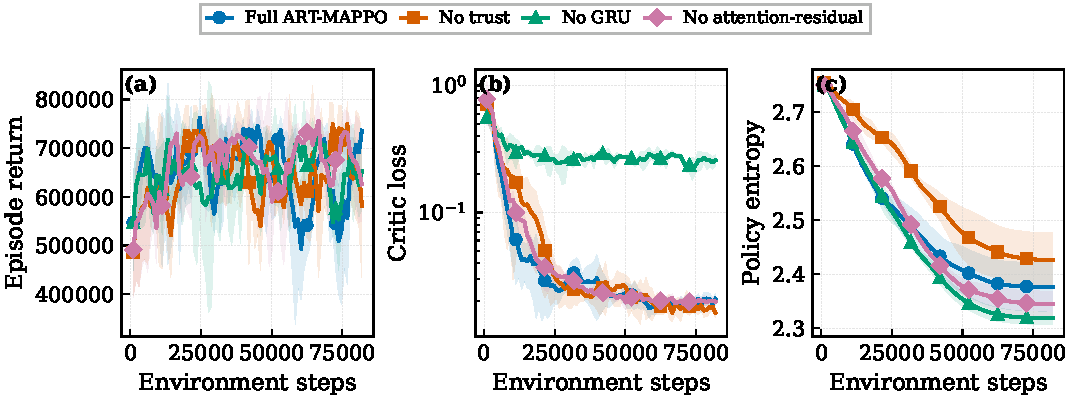
\includegraphics[width=\columnwidth]
{figures_v10/ablation_training_case1_v10.pdf}
\caption{Training-level component ablation in Case~1: episode return, Critic
Loss, and Policy Entropy. Curves and shaded regions denote the three-seed mean
and standard deviation, respectively.}
\label{fig:ablation_training_case1}
\end{figure}

\begin{figure}[!t]
\centering
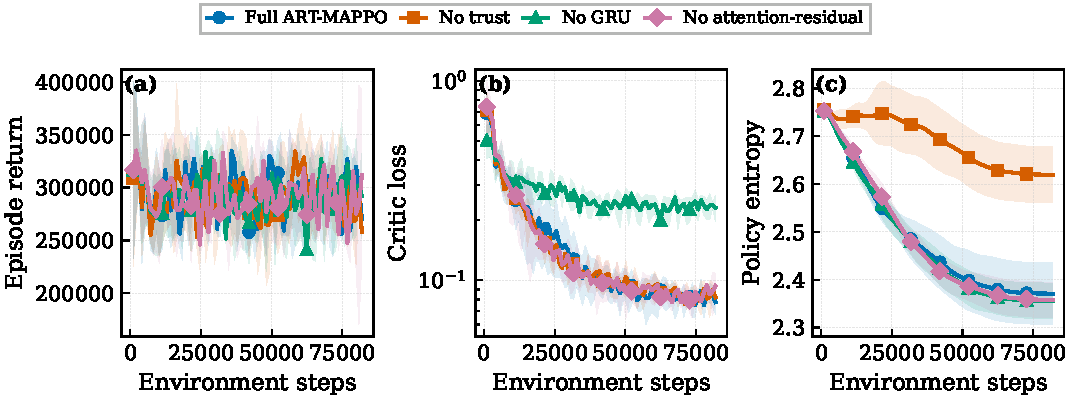
\includegraphics[width=\columnwidth]
{figures_v10/ablation_training_case2_v10.pdf}
\caption{Training-level component ablation in Case~2: episode return, Critic
Loss, and Policy Entropy. Curves and shaded regions denote the three-seed mean
and standard deviation, respectively.}
\label{fig:ablation_training_case2}
\end{figure}

The trust-aware mechanism is first interpreted from its intended role in the
proposed method. It is a training-time memory that changes the probability of
selecting tactical guidance, probing, and random actions according to
standardized episodic returns; it is disabled at deployment. Removing it
increases the final Policy Entropy from 2.3773 to 2.4287 in Case~1 and from
2.3722 to 2.6213 in Case~2. Its downstream effect is especially visible in
Case~1, where strict cooperative success decreases from 53\% to 29\%, even
though both variants retain 100\% target coverage and 100\% all-defender
interception. We therefore attribute the 24-percentage-point difference to
the training distribution induced by trust modulation, rather than to an
additional test-time controller. The no-trust variant does have a higher
final Case-1 return window, so the evidence does not imply that trust improves
every training statistic.

The GRU and attention--residual backbone operate during both optimization and
deployment. Removing the GRU increases the final-window Critic Loss from
0.01970 to 0.25320 in Case~1 and from 0.08222 to 0.23335 in Case~2, i.e.,
by factors of approximately 12.85 and 2.84. This confirms its strong role in
temporal value fitting. However, the no-GRU actor obtains 99\% cooperative
success in Case~1 compared with 53\% for the full actor. Thus, under the
present nearly Markovian observations and finite training budget, the
optimization advantage of recurrence does not translate into a higher
frozen-policy coordination rate. We report this distinction explicitly rather
than claiming a universal deployment advantage.

\begin{table}[!t]
\centering
\caption{Frozen-policy component ablation over 100 paired Monte Carlo
episodes per method and case.}
\label{tab:art_mappo_ablation}
\setlength{\tabcolsep}{3.0pt}
\begin{tabular}{llccc}
\hline
Case & Method & Coverage & All hit & Cooperation\\
     &        & (\%) & (\%) & (\%)\\
\hline
1 & Full ART-MAPPO & 100 & 100 & 53\\
1 & No trust       & 100 & 100 & 29\\
1 & No GRU         & 100 & 100 & 99\\
1 & No attention--residual & 100 & 100 & 2\\
\hline
2 & Full ART-MAPPO & 79 & 6 & 0\\
2 & No trust       & 79 & 5 & 0\\
2 & No GRU         & 80 & 5 & 0\\
2 & No attention--residual & 80 & 8 & 0\\
\hline
\end{tabular}
\end{table}

\begin{figure}[!t]
\centering
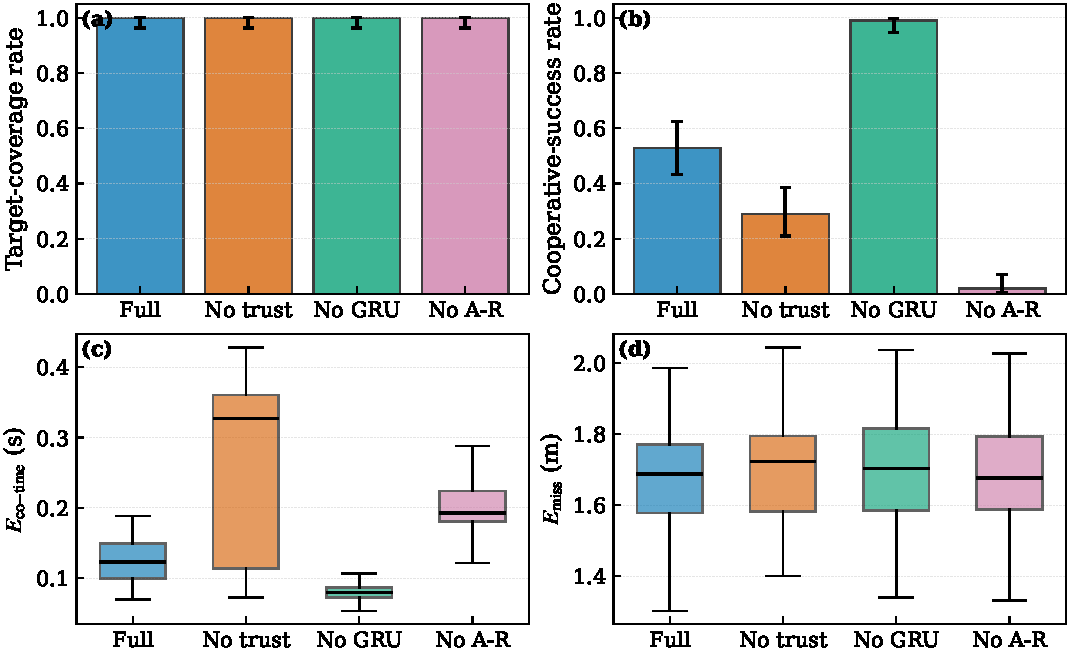
\includegraphics[width=\columnwidth]
{figures_v10/ablation_monte_carlo_case1_v10.pdf}
\caption{Frozen-policy component ablation in Case~1. Bars show
target-coverage and cooperative-success rates with 95\% Wilson intervals;
boxplots show the unmodified episode-level terminal metrics.}
\label{fig:ablation_monte_carlo_case1}
\end{figure}

Replacing the attention--residual backbone with the capacity-matched MLP
reduces Case-1 cooperative success from 53\% to 2\%, a
51-percentage-point difference, and increases mean
$E_{\mathrm{co\text{-}time}}$ from 0.1757 to 0.2395~s. Because the model
sizes are almost identical, this comparison isolates the value of structured
channel interaction and residual preservation beyond raw parameter count.

\begin{figure}[!t]
\centering
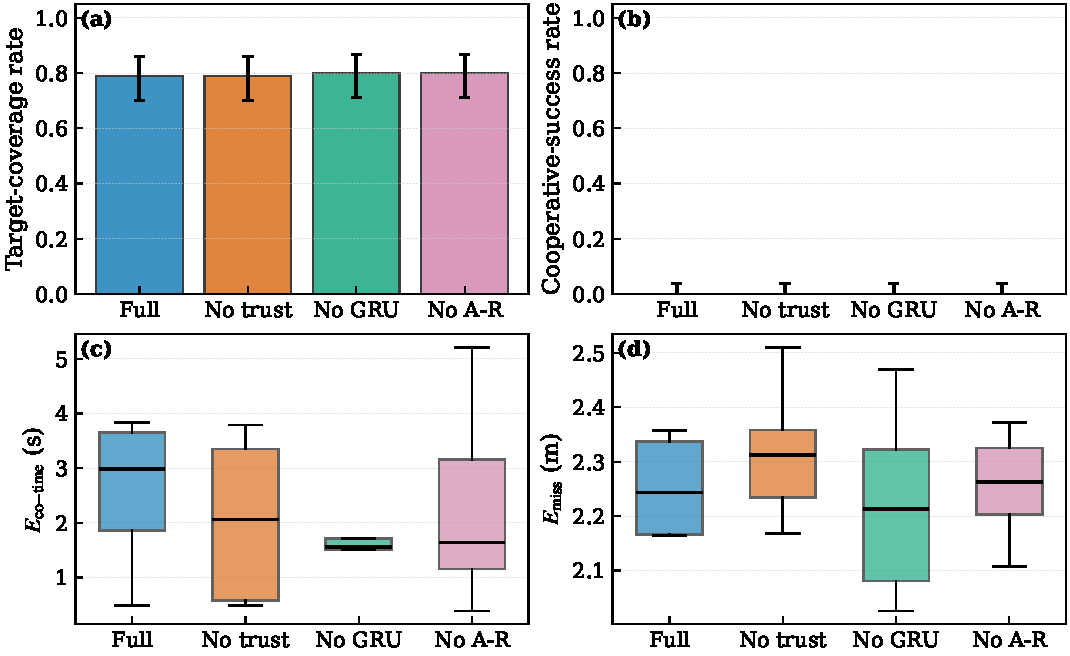
\includegraphics[width=\columnwidth]
{figures_v10/ablation_monte_carlo_case2_v10.pdf}
\caption{Frozen-policy component ablation in Case~2. The continuous metrics
are defined only for the 5--8 episodes per method in which all assigned
interceptors complete their engagements.}
\label{fig:ablation_monte_carlo_case2}
\end{figure}

Case~2 exposes a common limitation of all four models at the present training
budget. Target coverage is 79--80\%, only 5--8\% of episodes achieve
all-defender interception, and no variant satisfies the strict all-group
0.5-s coordination criterion. Accordingly, its terminal boxplots are treated
as diagnostics based on the small complete-episode subset, rather than as
evidence of component superiority. Overall, the experiment supports the
independent Case-1 contributions of trust-aware training and structured
attention--residual processing, demonstrates the GRU's strong contribution to
critic fitting, and delineates the conditions under which these optimization
effects do not translate into strict deployment success.
